\chapter{Wyniki badań}

Treść rozdziału trzeciego --- prezentacja i~analiza wyników badań.

\section{Analiza wyników}

Opis uzyskanych wyników wraz z~odniesieniami do tabel, rycin i~wykresów.

Przykład odniesienia do wykresu --- patrz (Wykres~\ref{wyk:przyklad}).

\begin{wykres}[htbp]
  \caption{Rozkład odpowiedzi respondentów według kategorii}\label{wyk:przyklad}
  \centering
  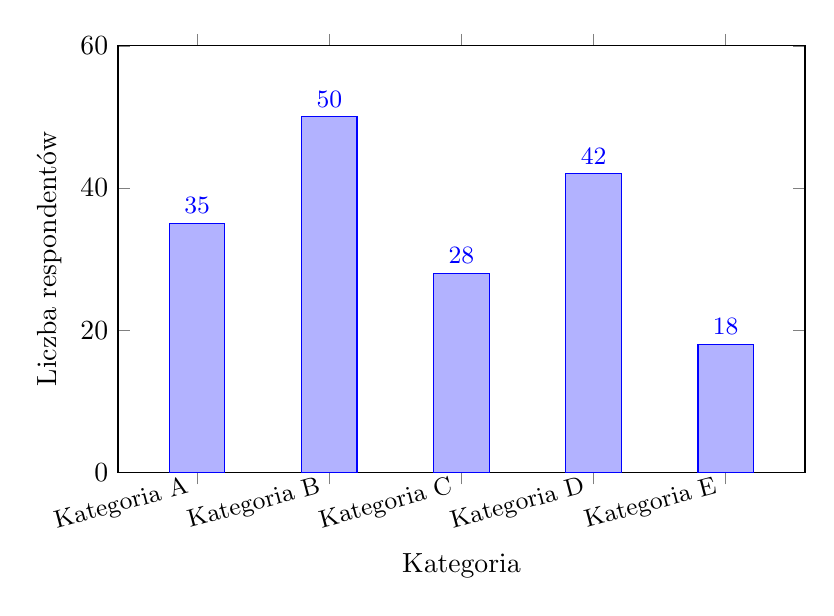
\begin{tikzpicture}
    \begin{axis}[
      ybar,
      width=0.85\textwidth,
      height=7cm,
      bar width=20pt,
      ylabel={Liczba respondentów},
      xlabel={Kategoria},
      symbolic x coords={Kategoria A,Kategoria B,Kategoria C,Kategoria D,Kategoria E},
      xtick=data,
      x tick label style={rotate=15, anchor=east, font=\small},
      ymin=0,
      ymax=60,
      nodes near coords,
      every node near coord/.style={font=\small},
      enlarge x limits=0.15,
    ]
      \addplot coordinates {
        (Kategoria A, 35)
        (Kategoria B, 50)
        (Kategoria C, 28)
        (Kategoria D, 42)
        (Kategoria E, 18)
      };
    \end{axis}
  \end{tikzpicture}
  \zrodlo{badania własne.}
\end{wykres}

\section{Omówienie wyników}

Dyskusja nad uzyskanymi wynikami i~ich interpretacja w~kontekście literatury.
